\chapter{Results}
The results stem from a common configuration pattern for both SKLearn and Keras, aswell as distinct parametrization of algorithms for each.
The training set is reduced from 50000 to 12500 datapoints, while the test set is reduced from 10000 to 2500. The reduction was deemed necessary to ensure
adequate expenditure of time for the algorithms. 

Notably, the displayed values are one of many produced results and may vary from execution to execution.
The different computational approaches can be found in the accompanying IPYNB/PY files, located in the ''src'' directory of the repository.
All aggregated results can be found in the ''log'' directories, each produced from a linux-system and a windows-system with hardware specifications as depicted
in the projects ''README.md''

\section{Keras neural network}
The Keras-driven neural network is the main focus of the experimentation. There are three main phases during the algorithm.

First we create a standard, sequential model for basic information gathering, that also serves as a 
reliable reference for further approaches. The basic model always uses the same parameters and layers.

Secondly, we run hyperparameter evaluation using the \href{https://keras.io/keras_tuner/}{keras\_tuner} library, to find models that are 
more accurate. The model resembles the standard model, with deviations in activation functions, dropout and learning rates and units in the dense layer, as well as randomized deactivation of whole layer structures.
While almost every aspect of the model can be adjusted (see Overengineered Model), the more fundamental approach (Hypermodel) allowed for better training times while being similarly efficient in it's search.
The Hypermodel is used for the strategy of Random Search, Bayesian Optimization and \href{https://arxiv.org/abs/1603.06560}{Hyperband}

Thirdly, utilizing the findings by the hyperparameter search, a model is created and trained using the most optimal setup found during the evaluation.
In the current implementation, the model with the highest accuracy score of the three mentioned strategies is chosen.

For reference, the optimized model for the following results were automatically assigned by the algorithm, which is the Hyperband-Search (Trial 12) on the Windows device.
It uses the following configuration:
\begin{center}
  \begin{verbatim}
    Standard Model    |    Optimal Model
    ------------------+--------------------
    Conv2D(relu)      | Conv2D(relu)
    Conv2D(relu)      | Conv2D(relu)
    MaxPooling2D      | 
    Dropout(0.25)     | 
    Flatten()         | Flatten()
    Dense(256,relu)   | Dense(480,sigmoid)
    Dense(256,relu)   | Dense(480,sigmoid)
    Dense(10,softmax) | Dense(10,sigmoid)
    ------------------+---------------------
    lr:       0.0001  |  0.001   
  \end{verbatim}
\end{center}

\begin{table}[H]
  \centering
  \begin{tabular}{|l|l|l|l|l|}\hline
                        & \multicolumn{2}{|c|}{Standard Model}    & \multicolumn{2}{|c|}{Optimized Model} \\\hline
      Training time     & \multicolumn{2}{|l|}{99.97050666809082s} & \multicolumn{2}{|l|}{114.58384299278259s}\\\hline\hline
      Model             & \multicolumn{1}{|c|}{Dataset} & \multicolumn{1}{|c|}{Exec. Time}          & \multicolumn{1}{|c|}{Accuracy}            & \multicolumn{1}{|c|}{Loss} \\\hline
      Standard Model    & Train   & 1.7971601486206055  & 0.5135221481323242  & 1.3555371761322021 \\
      Optimized Model   & Train   & 1.5238370895385742  & 0.8758201599121094  & 0.4363606870174408 \\
      Standard Model    & Test   & 0.3897683620452881  & 0.4715772569179535  & 1.470583200454712 \\
      Optimized Model   & Test   & 0.40241503715515137  & 0.5268214344978333  & 1.4896273612976074 \\\hline
    \end{tabular}
  \caption{Training time, validation time, accuracy and loss for the standard and the optimized neural network model.}
  \label{tab:std_opt_model_comparison}
\end{table}

\begin{table}[H]
  \centering
  \begin{tabular}{|l|l|l|l|}\hline
    \multicolumn{1}{|c|}{Log} & \multicolumn{1}{|c|}{HPS Strategy}   & \multicolumn{1}{|c|}{Accuracy} & \multicolumn{1}{|c|}{Loss} \\\hline
    WIN & Random Search           & 0.46357086300849915 & 1.4989255666732788 \\
    LNX & Random Search           & 0.40512409806251526 & 1.7340798377990723 \\
    WIN & BayesianOptimization    & 0.5212169885635376  & 1.5947179794311523 \\
    LNX & BayesianOptimization    & 0.3010408282279968  & 6.0242438316345215 \\
    WIN & Hyperband               & 0.5004003047943115  & 1.6119012832641602 \\
    LNX & Hyperband               & 0.5252201557159424  & 1.8868718147277832 \\\hline
  \end{tabular}
  \caption{Small excerpt of the hyperparameter evaluation logs -- Each strategy and their best performances on accuracy and loss for each machine.}
  \label{tab:hps_strategy_comparison}
\end{table}
Surprisingly, the Bayesian Optimization strategy on linux appeared to have major issues for reasons not further investigated, while it competes well on windows.
Given the size limit of this report, please refer to the hyperparameter-tuning-log.txt files for concise information on all strategies and their models.

The following visualizations further aid the understanding of the results and depict the difference in model fitting -- the optimized 
variant reaches a high point of validation accuracy very fast but does not improve afterwards.
Given the difference in training and validation, this may indiciate overfitting.
\begin{figure}[H]
  \centering
  \begin{minipage}{.5\textwidth}
    \centering
    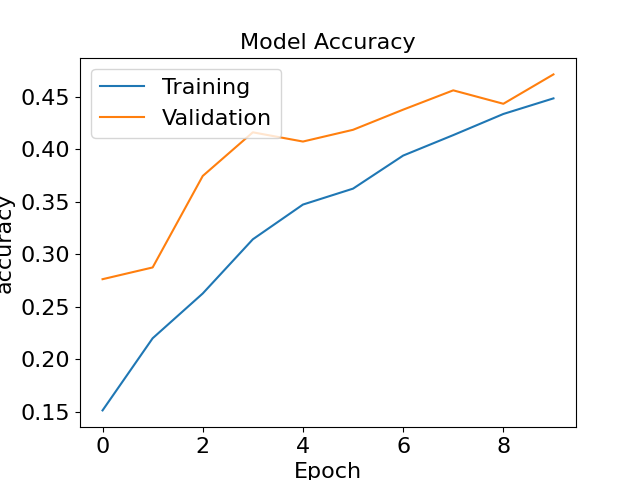
\includegraphics[width=1.0\linewidth]{img/training_history_standard.png}
    \label{fig:training_history_standard}
  \end{minipage}%
  \begin{minipage}{.5\textwidth}
    \centering
    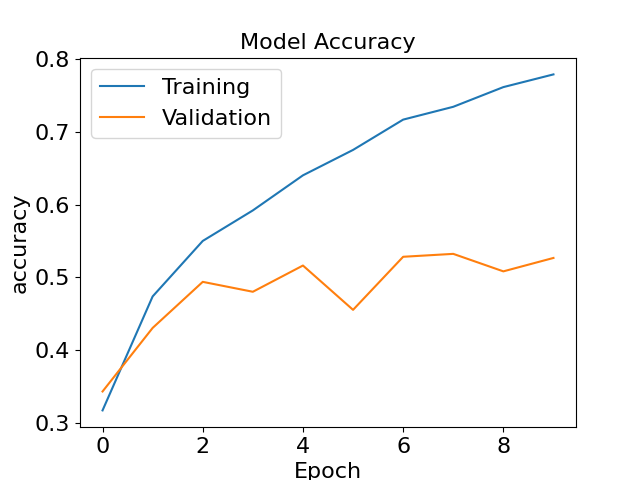
\includegraphics[width=1.0\linewidth]{img/training_history_optimal.png}
    \label{fig:training_history_optimal}
  \end{minipage}
  \caption{Training accuracy score comparison inbetween default network (left) and optimized network (right) parametrization.}
  \label{fig:training_history_overview}
\end{figure}

% Overfeed linewidth for better readability
\begin{figure}[H]
    \centering
    \begin{minipage}{.5\textwidth}
      \centering
      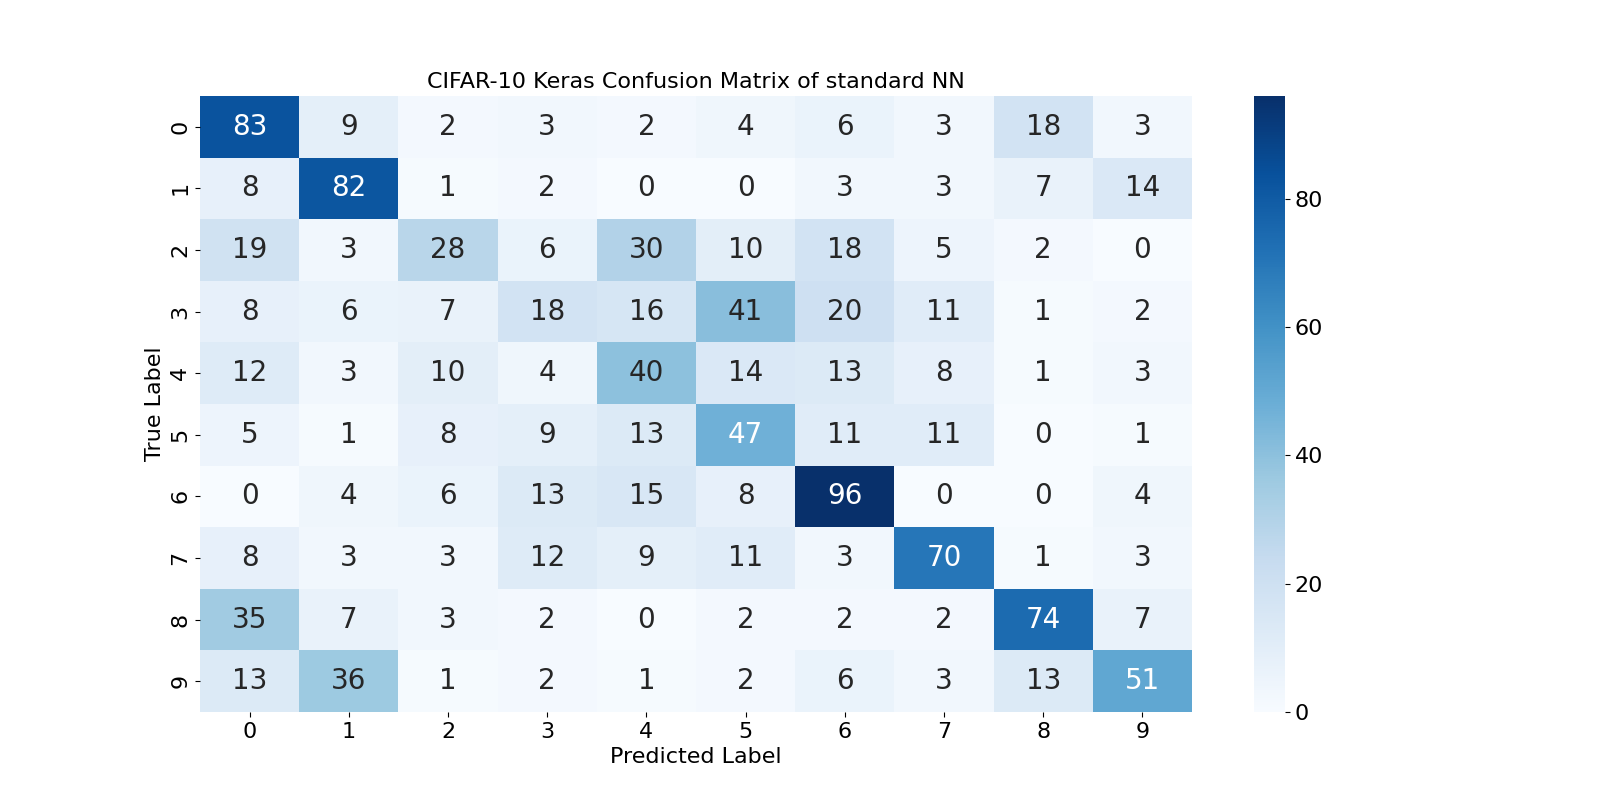
\includegraphics[width=1.25\linewidth]{img/ConfusionMatrix_standard.png}
      \label{fig:confusion_matrix_standard}
    \end{minipage}%
    \begin{minipage}{.5\textwidth}
      \centering
      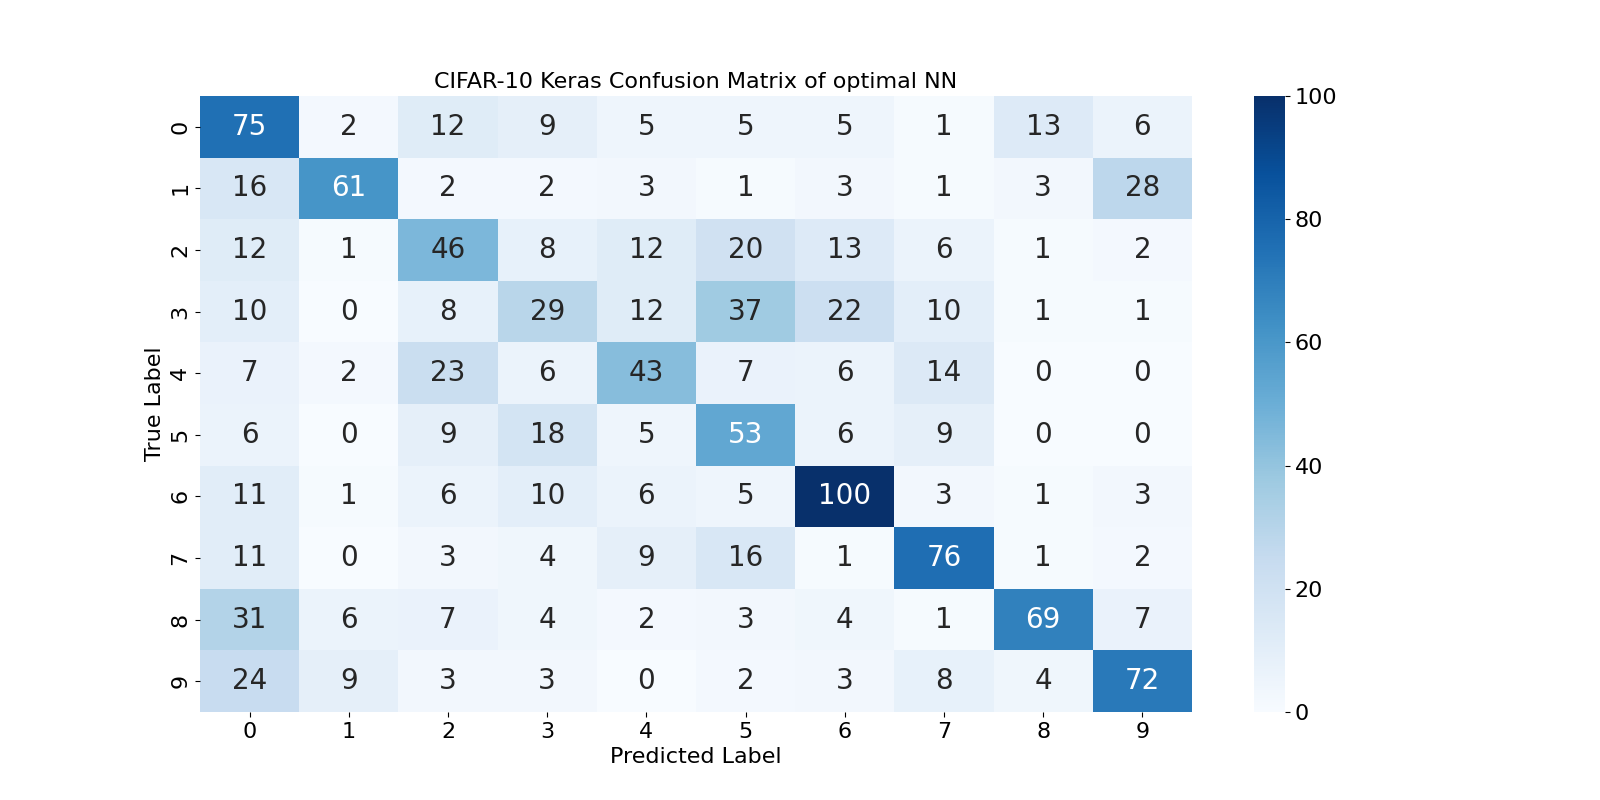
\includegraphics[width=1.25\linewidth]{img/ConfusionMatrix_optimal.png}
      \label{fig:confusion_matrix_optimal}
    \end{minipage}
    \caption{Confusion matrix comparison inbetween default network (left) and optimized network (right) parametrization.}
    \label{fig:confusion_matrix_overview}
\end{figure}

\section{SKLearn multi-layer perceptron}
To further investigate the performance on the CIFAR10 dataset, we utilize the multi-layer perceptron of the SKLearn library to add an additional viewpoint on training and testing.


